
\section{Kết quả huấn luyện}

\subsection{So sánh các mô hình}

Trong quá trình nghiên cứu, chúng tôi đã thử nghiệm với nhiều kiến trúc mô hình khác nhau. 
Bảng \ref{tab:model_performance} trình bày kết quả so sánh hiệu suất của các mô hình.

\begin{table}[h]
\centering
\caption{So sánh hiệu suất của các mô hình}
\label{tab:model_performance}
\begin{tabular}{|l|c|c|c|}
\hline
\textbf{Mô hình} & \textbf{accuracy tốt nhất} & \textbf{Epoch tốt nhất} & \textbf{Loss tốt nhất} \\
\hline
MobileNetV3Small_NotFreezed & 0.9139 & 17 & 0.2162 \\
\hline
MobileNetV3Small_Freezed & 0.8758 & 4 & 0.3322 \\
\hline
MobileNetV3Small_Freezed2 & 0.8495 & 18 & 0.3757 \\
\hline
ModelB & 0.7030 & 2 & 0.8094 \\
\hline
ModelA & 0.6762 & 4 & 1.0114 \\
\hline

\end{tabular}
\end{table}

\subsection{Phân tích kết quả}


Từ kết quả thực nghiệm, chúng tôi nhận thấy:

\begin{itemize}
  \item Mô hình có accuracy cao nhất là \textbf{MobileNetV3Small_NotFreezed} với accuracy \textbf{0.9139}.
  \item accuracy trung bình của các mô hình: \textbf{0.8037 $\pm$ 0.1070}.
  \item Thời gian hội tụ trung bình (epoch): \textbf{9.0}.
\end{itemize}

\subsection{Biểu đồ so sánh}

\begin{figure}[h]
  \centering
  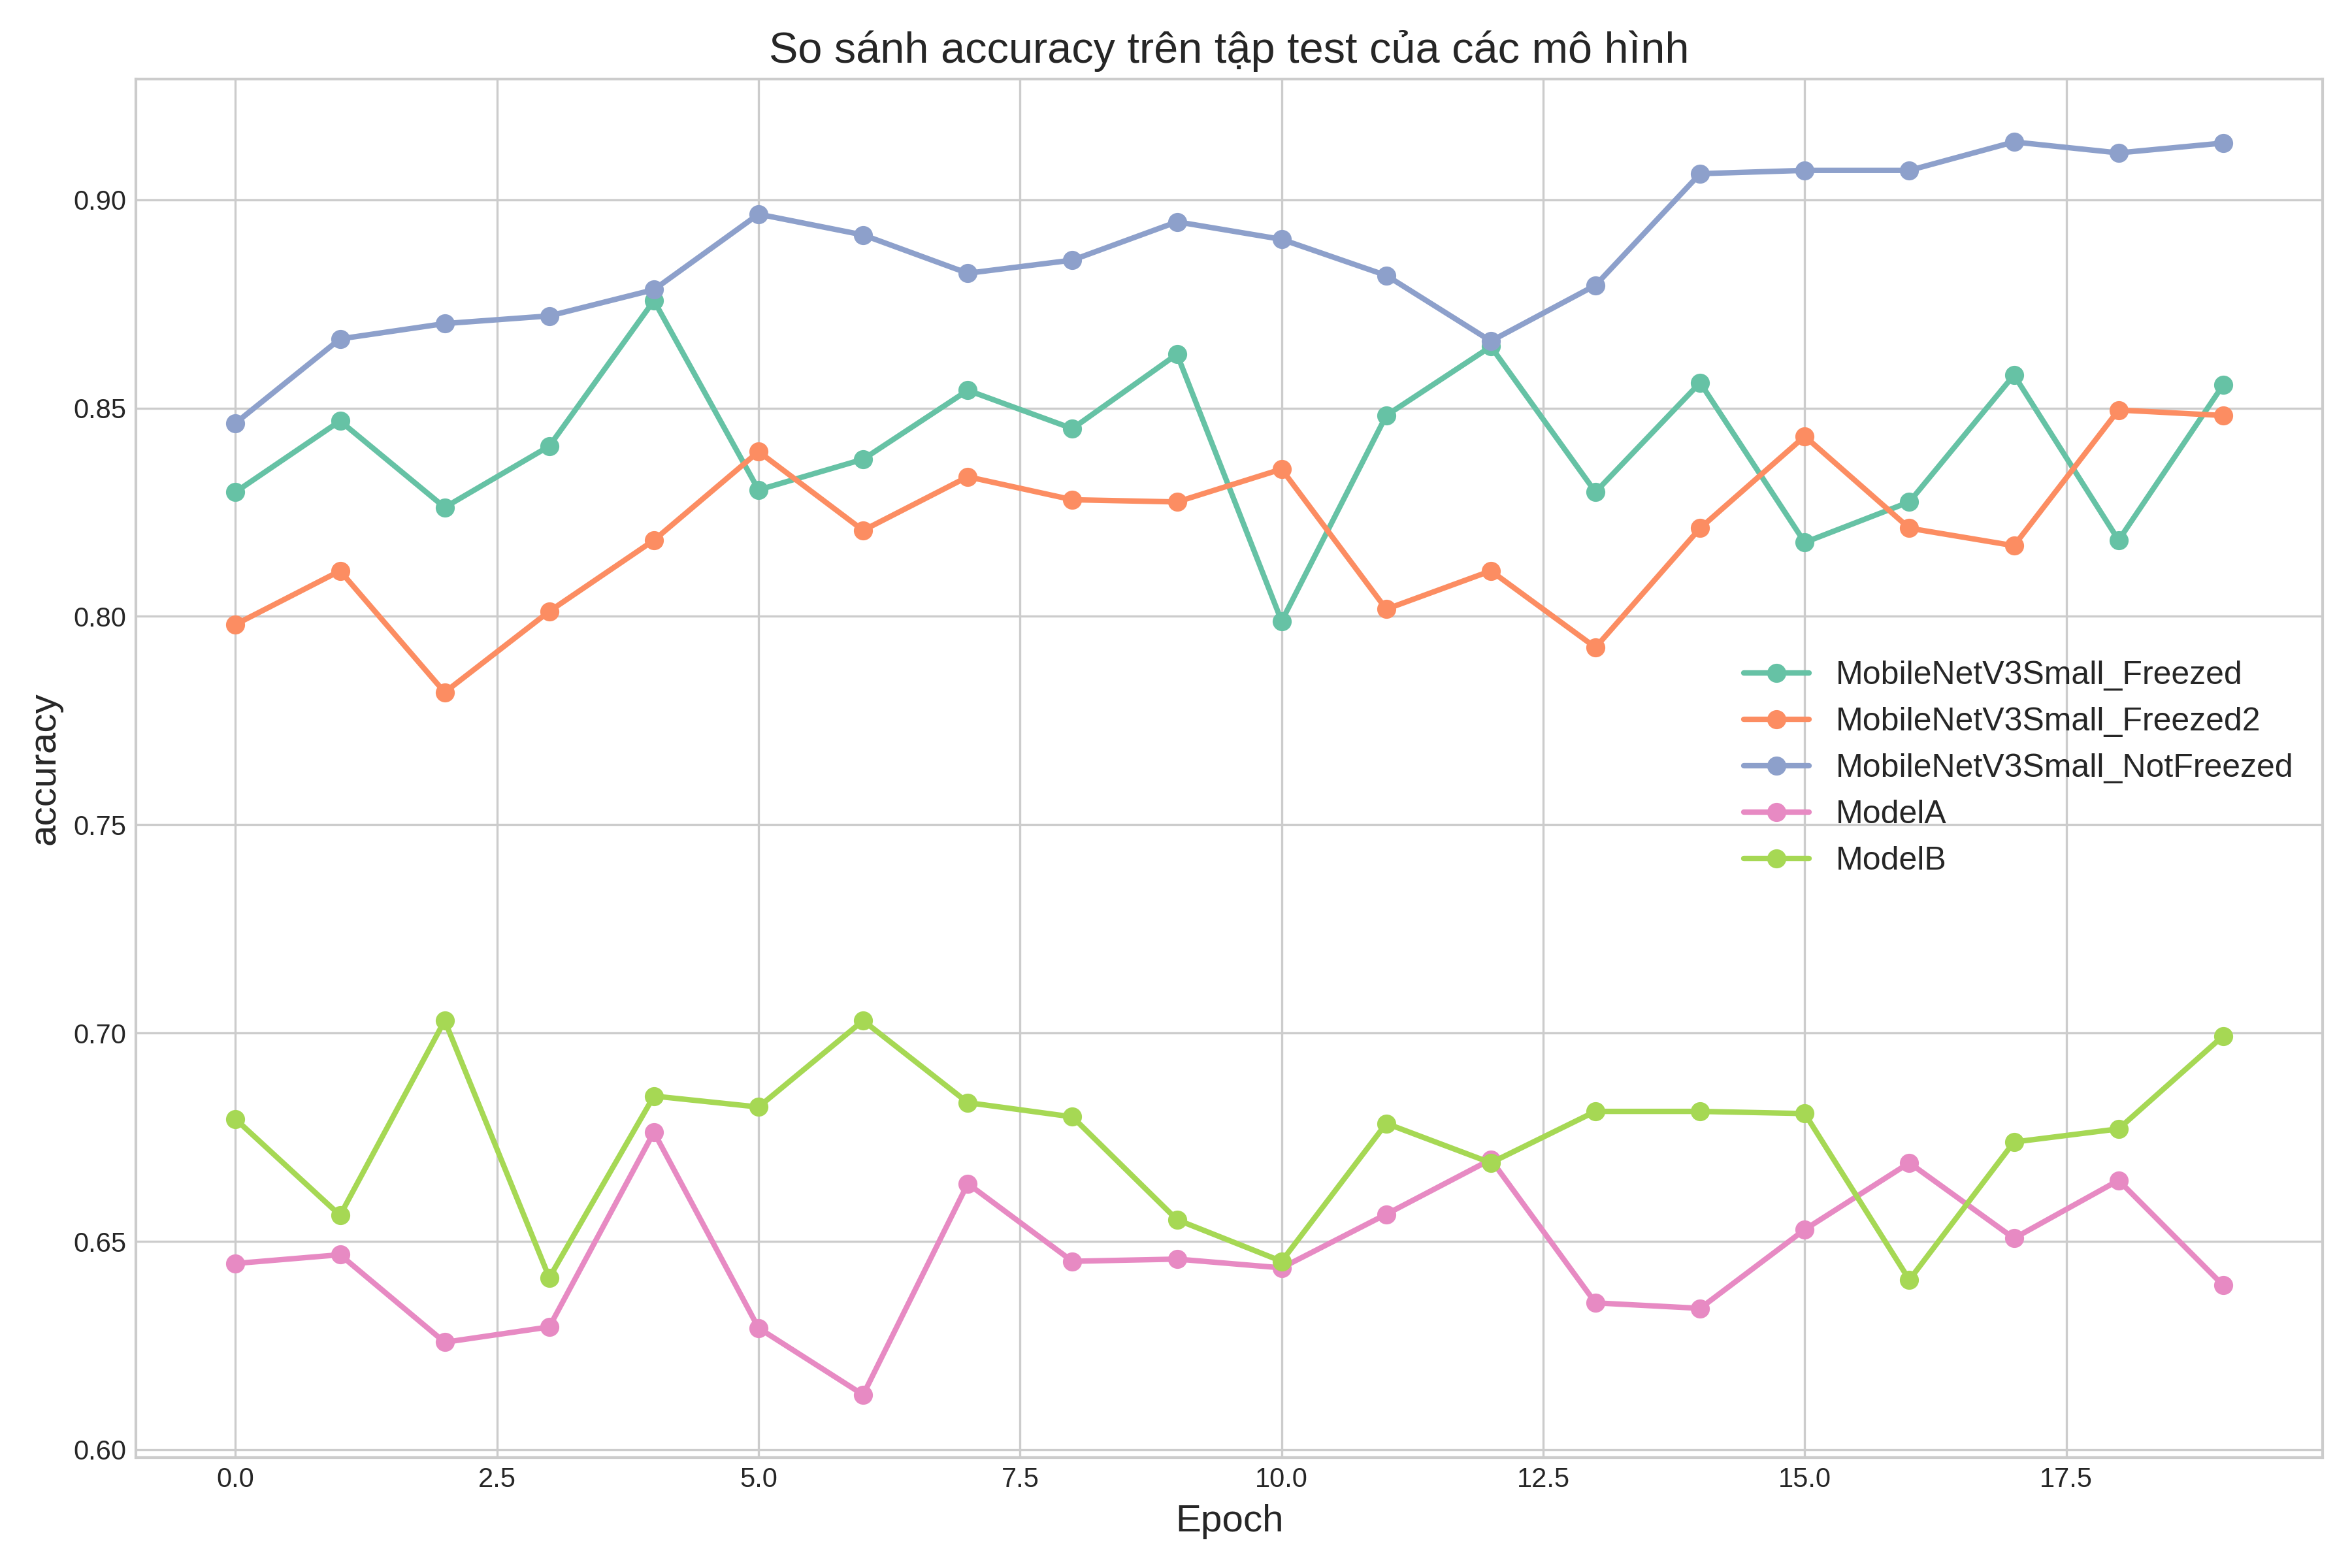
\includegraphics[width=0.8\textwidth]{analysis_results/test_accuracy_comparison.png}
  \caption{So sánh accuracy trên tập test của các mô hình}
  \label{fig:test_accuracy}
\end{figure}

\begin{figure}[h]
  \centering
  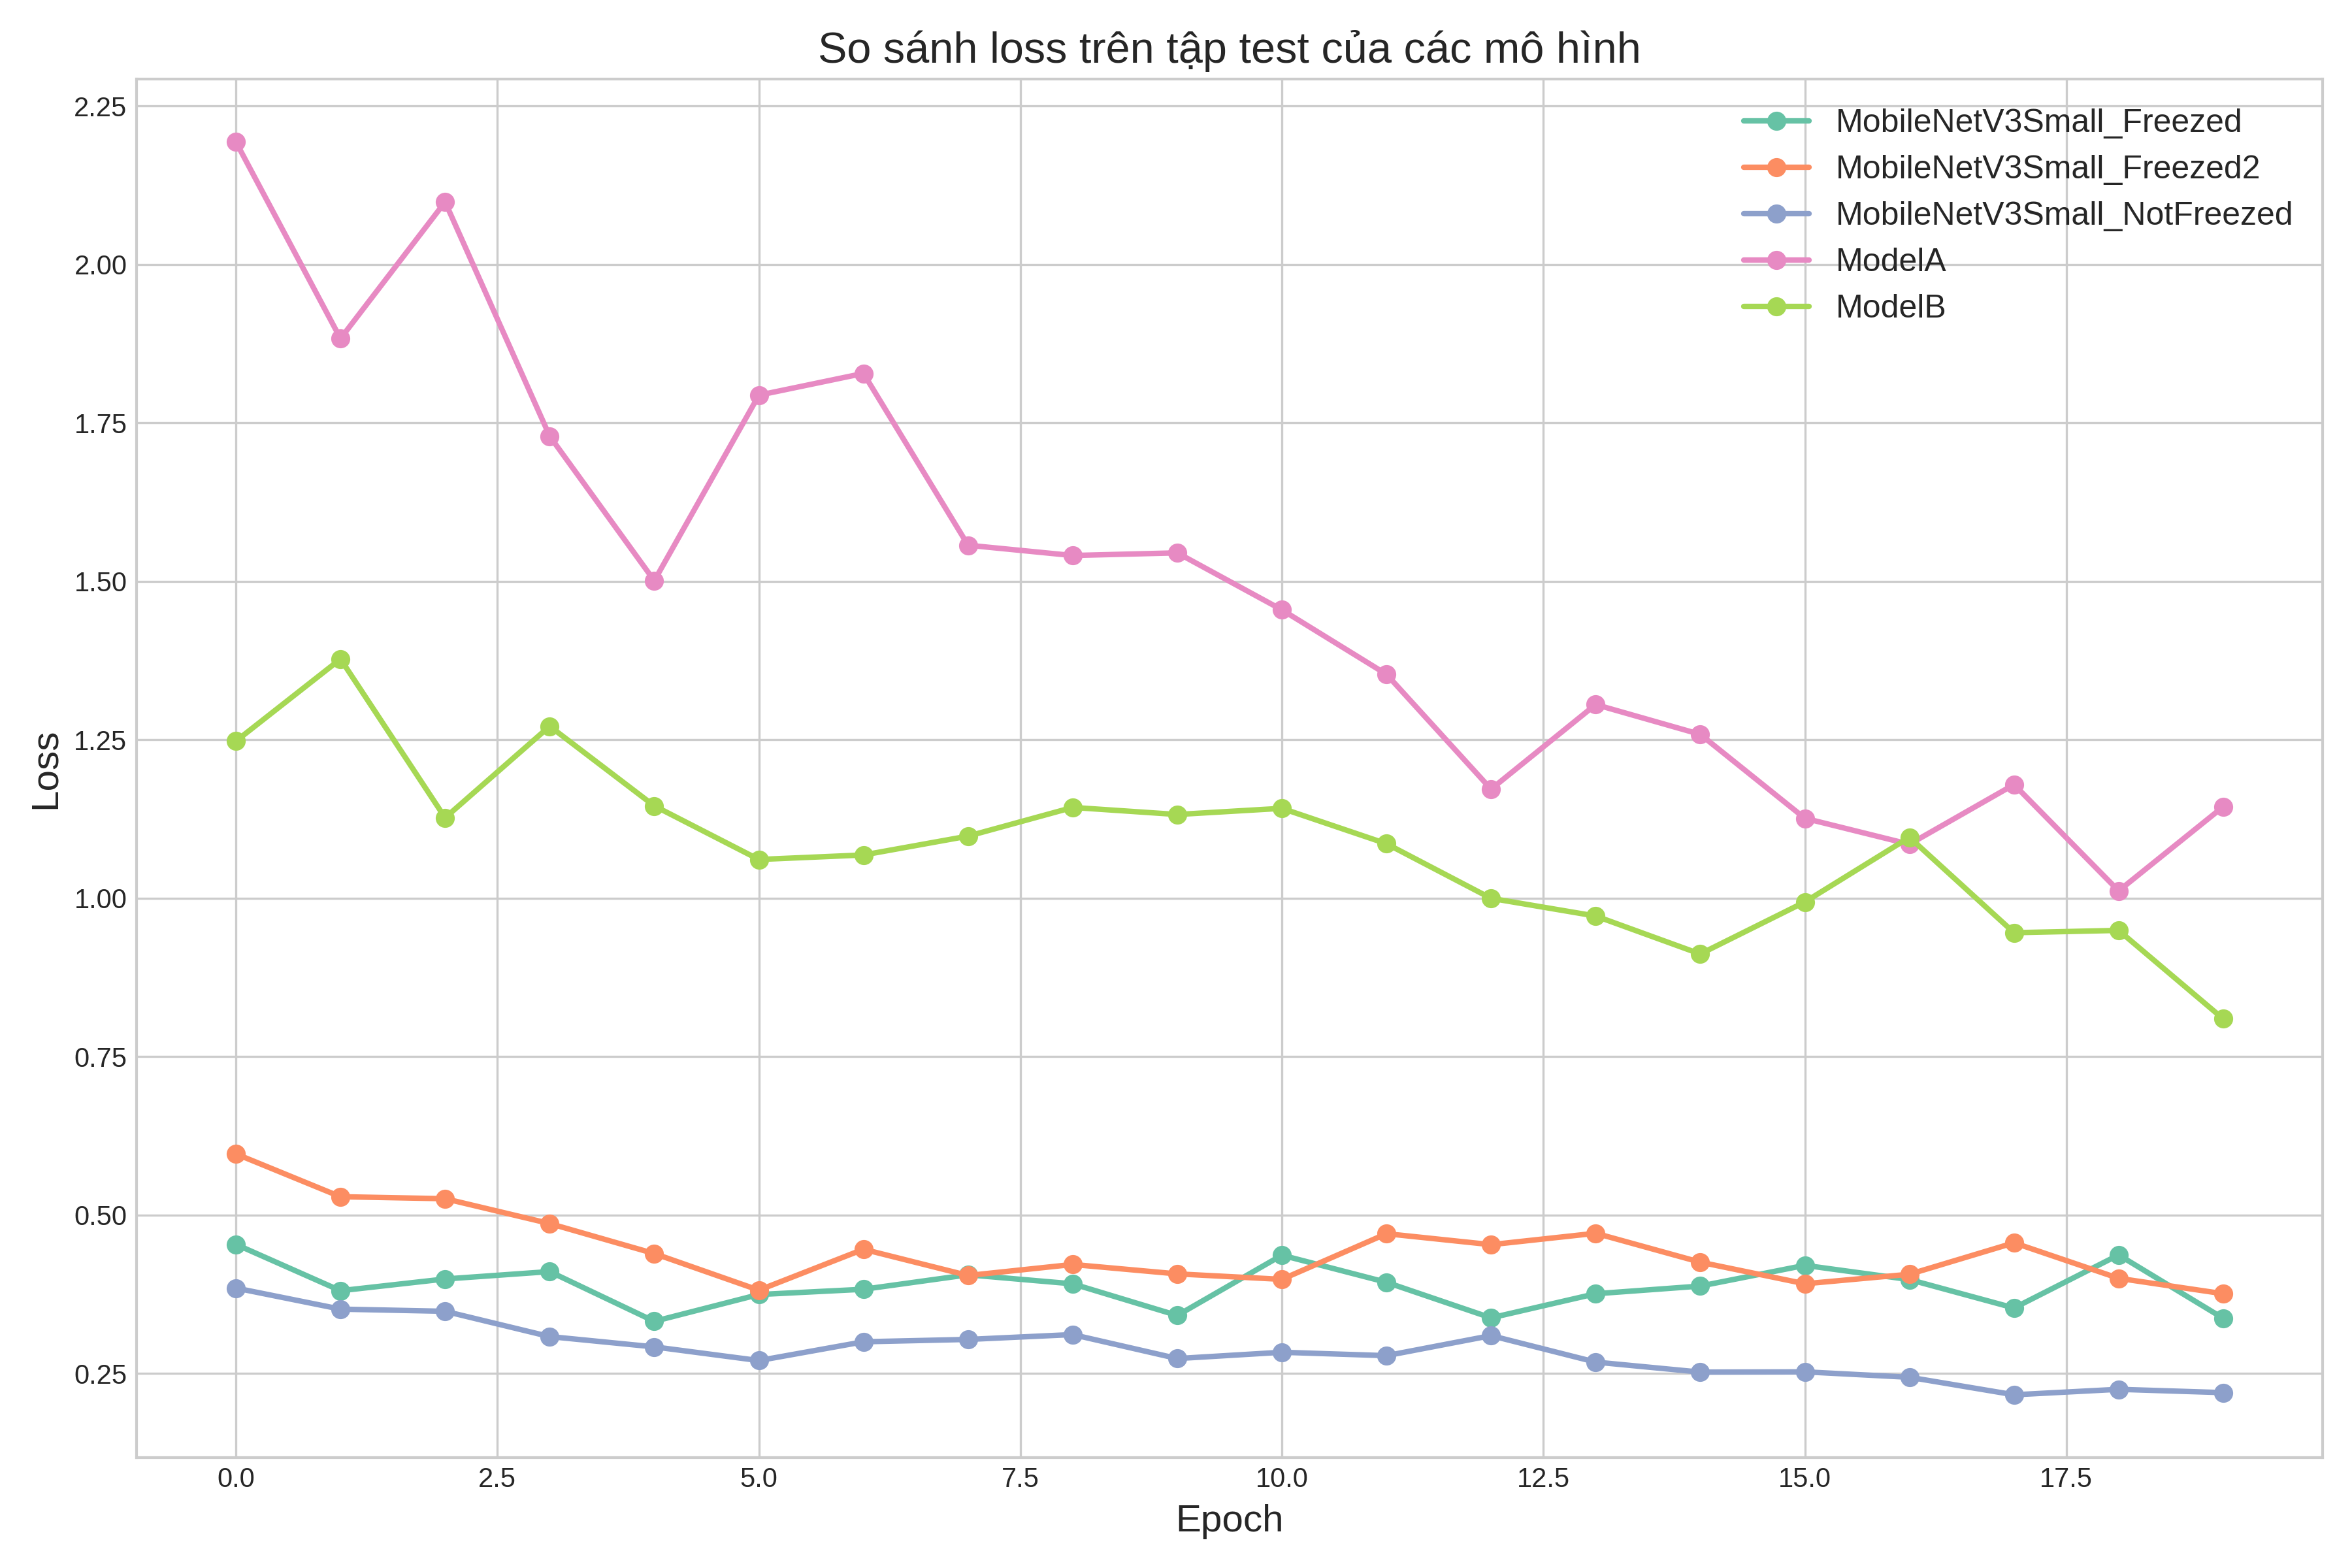
\includegraphics[width=0.8\textwidth]{analysis_results/test_loss_comparison.png}
  \caption{So sánh loss trên tập test của các mô hình}
  \label{fig:test_loss}
\end{figure}

\begin{figure}[h]
  \centering
  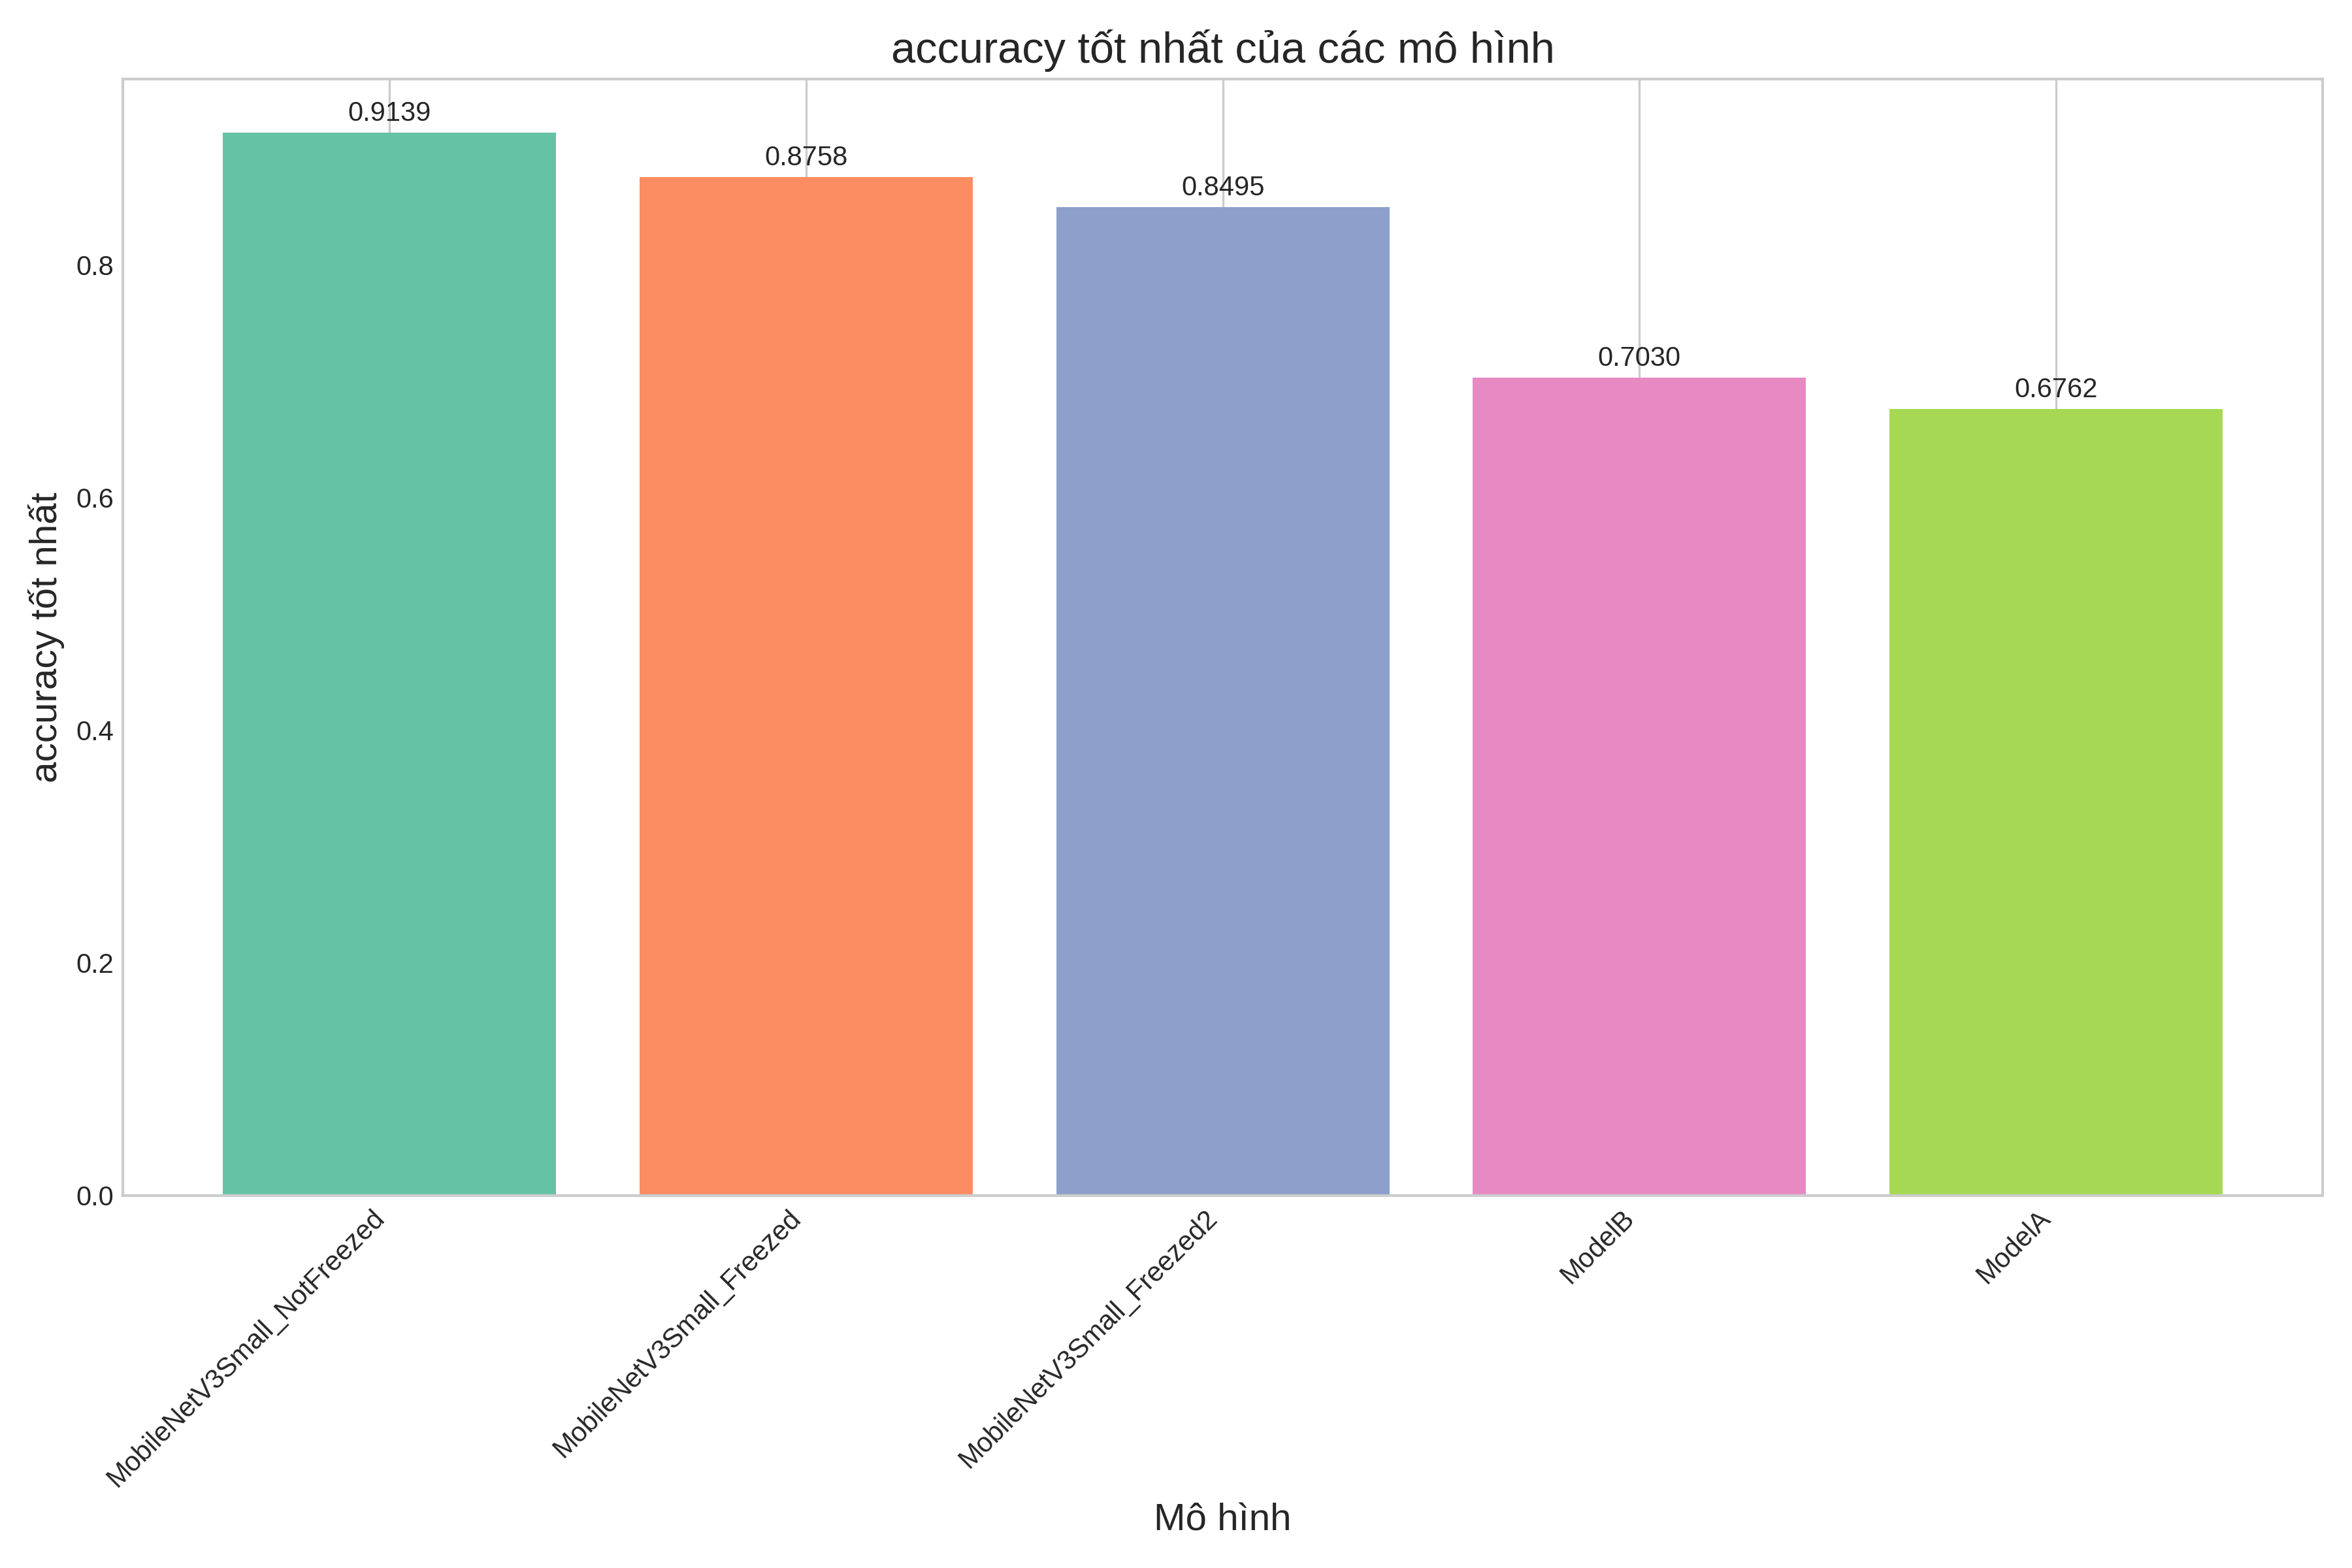
\includegraphics[width=0.8\textwidth]{analysis_results/best_accuracy_comparison.png}
  \caption{So sánh accuracy tốt nhất của các mô hình}
  \label{fig:best_accuracy}
\end{figure}
